\xchapter{Discussão}{}
\label{discussao}


Respostas para perguntas gerais. Fazer uma seção para cada.
Cuidado com a questão das funcionalidades de cada tool -- pode ser o motivo de ser mais usada,
mesmo que não seja sustentável.

\section{Questões} 

Uma questão interessante é a de ``integridade''. 
O que acontece com os resultados anteriores (publicados)
se houver um erro ou uma mudança substancial da forma de calcular algo?
Na prática, só deveríamos permitir refactorings no código 
de um software acadêmico ou adição de novas funcionalidades?
(Chris)

An so what?

O ecossistema de software acadêmico de análise estática sofre de disfunctional ...?

%Encarar o software acadêmico como a "plataforma" do ecossistema de software.
%Pensar no ecossistema de pesquisa e produção intelectual.

Não encontramos relação entre disponibilidade de download e menções, seja Cita, Usa ou Contribui.

\subsection{Q1 - \QuestaoUm}

... a Figura \ref{mentions-by-year} (a) é possível notar uma clara relação
entre o número total de menções e o número de projetos novos por ano, ou seja,
ao subir o número de projetos sobe também, numa proporção muito maior, o número
de menções. Quanto mais projetos mais menções, mas também o número de menções
a software de modo geral cresce ...

... a Figura \ref{mentions-by-year} (b) apresenta o número de menções por tipo Cita, Usa e Contribui ao
ano onde é possível notar que ambos os tipos apresentam crescimento similar ao longos dos anos ...

\begin{figure}[h]
  \begin{minipage}{0.5\textwidth}
    \centering
    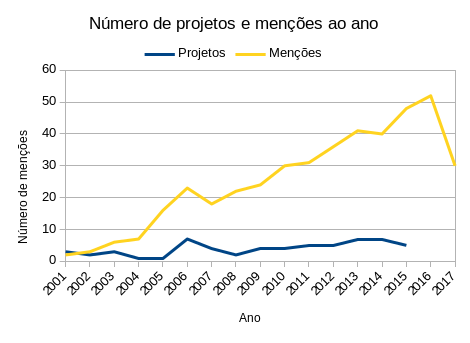
\includegraphics[scale=0.6]{imagens/mentions-projects-by-year.png}
    \texttt{(a)}
  \end{minipage}
  \begin{minipage}{0.5\textwidth}
    \centering
    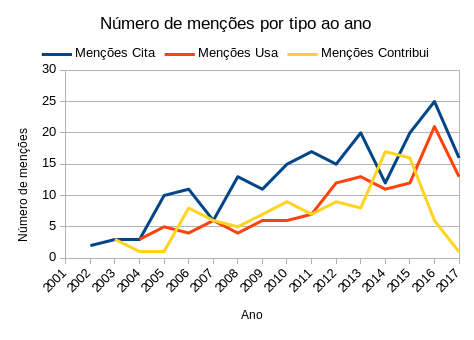
\includegraphics[scale=0.6]{imagens/mentions-type-by-year.png}
    \texttt{(b)}
  \end{minipage}
  \caption{Número total de (a) menções e projetos ao ano e (b) menções por tipo ao ano.}
  \label{mentions-by-year}
\end{figure}

... a Figura \ref{mentions-trend-without-projects} mostra a taxa de crescimento
isolada do crescimento de projetos, utilizamos várias amostras de menções por
ano capturando grupos distintos de no máximo 3 projetos e as menções a estes projetos,
a taxa de crescimento média de menções ao longo dos anos é de 38\%, ou seja,
permanecendo constante o número de projetos ao ano, as menções irão crescer numa taxa
de 38\% ao ano na média ...

\begin{figure}[h]
  \center
  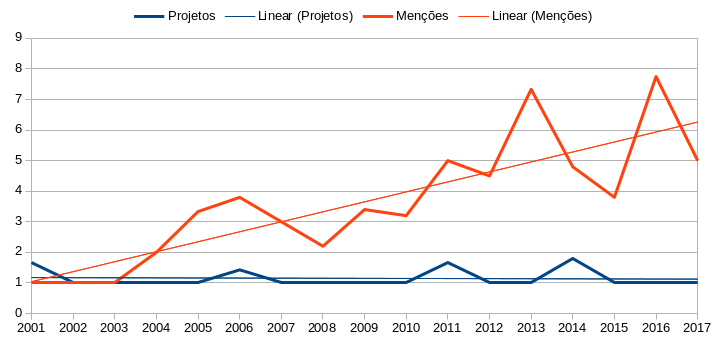
\includegraphics[scale=0.6]{imagens/mentions-trend-without-projects.png}
  \caption{Média de menções por ano em grupos de tuplas com número de projetos constante (maximo 2~3) ao ano.}
  \label{mentions-trend-without-projects}
\end{figure}

\subsection{Q2 - \QuestaoDois} % tamanho médio

O tamanho médio dos projetos é de 820 módulos, 22 projetos tiveram seus códigos
fontes analisados para extrair este dado, os demais projetos não tinham
código disponível. Esta média considera a última versão disponível em código
fonte de cada projeto.

O tamanho médio dos projetos em estágio inicial de desenvolvimento é de 595
(exclui os com valor = 0) são muito menor que osem estágio de evolução e
serviço  de 1261, ou seja, são pelo menos 2 vezes maior em número de módulos.

São 20 projetos em estágio inicial de desenvolvimento ao total, 12 foram
analisados em código fonte. São 8 projetos em estágio de evolução e serviço,
estes dois estágios foram agregados num único conjunto pois possuem características
próximas, e entre os únicos 2 em estágio de evolução (6 são serviço) estão
muito mais próximos do estágio de serviço que do estágio inicial. Todos os 8
tiveram código fonte analisado.

Número médio de módulos

\begin{figure}[h]
  \center
  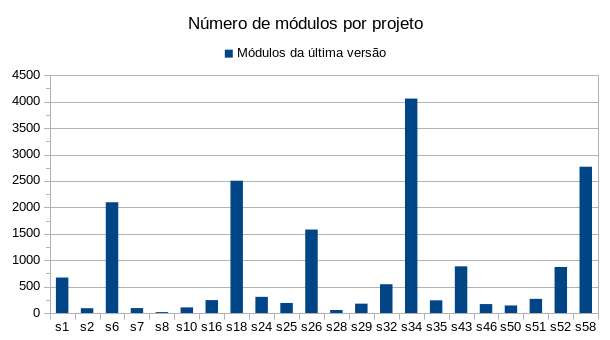
\includegraphics[scale=0.6]{imagens/modules-total.png}
  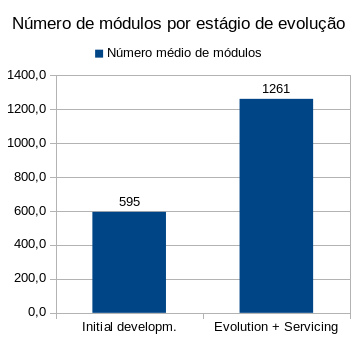
\includegraphics[scale=0.6]{imagens/modules-average.png}
  \caption{...}
  \label{modules-average}
\end{figure}

\subsection{Q3 - \QuestaoTres} % idade média

Para calcular idade foi considerados todos os anos em que houve lançamento
de versões e também todos os anos em que foram encontradas menções ao software,
entre todo o período encontrado para cada software, o primeiro ano onde uma
das ocorrências tenham acontecido, aquela mais antiga, foi considerada como
o nascimento do projeto, a partir dessa informação calculou-se a idade com
base o ano de 2017, ou seja, subtraimos 2017 do ano encontrado mais antigamente
para cada projeto de software.

Os projetos em estágio Servicing são entre 4 e 15 anos de idade.

A idade mínima de qualquer projeto é 2 anos, já que a revisão de literatura
para seleção dos projetos limitou-se ao ano de 2015, ou seja, não há entre
os projetos software mais recente do que 2015.

Idade VS lançamentos VS menções dos projetos em initial development.
Idade VS lançamentos VS menções dos projetos em Evolution e Servicing.

\begin{figure}[h]
  \centering
  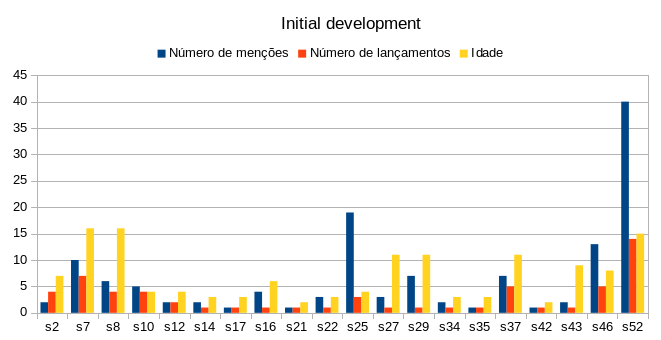
\includegraphics[scale=0.6]{imagens/age-initial-development.png}
  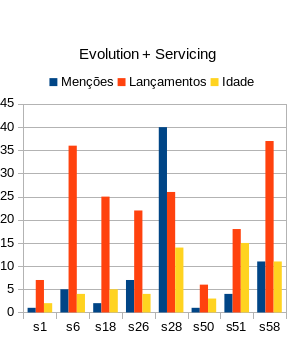
\includegraphics[scale=0.6]{imagens/age-evolution-servicing.png}

  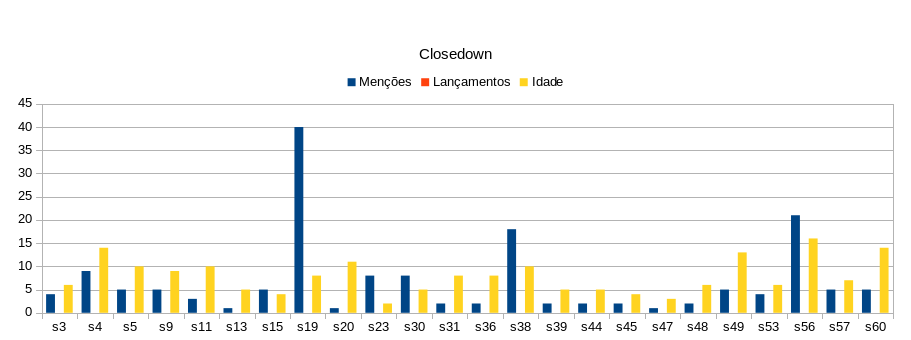
\includegraphics[scale=0.6]{imagens/age-closedown.png}
  \caption{Número de menções, lançamentos e idade de cada projeto por estágio de evoluçao.}
  \label{age-vs-stage}
\end{figure}

A idade dos projetos em initial são em todos os projetos superior ao número de
lançamentos, e na maioria superior também ao número de menções, os projetos
evolution+servicing tem natureza contrária onde o número de lançamentos é
sempre superior a idade, já o número de menções é superior ou inferior depender
do projeto. Os projetos em Closedown possuem idade superior ao número de
menções, apesar de existir casos contrário, entre estes casos destaque para os
projetos \texttt{s19}, \texttt{s38} e \texttt{s56} por possuírem número de
menções bem acima da média geral e também por possuir o número absoluto em
relação a idade grande, especialmente o software \texttt{s19} que possui número
de menções comparado a apenas dois outros projetos mas que encontram-se em
initial ou evolution e estão disponiveis para download, inclusive em código
fonte. Algp que este projeto \texttt{s19} não reflete.

Initial tem idade minima 2 (todos tem essa idade minima ja que a data limite na selecao foi 2015)

A média de idade é aproximadamente igual em todos os estágios de evolução (evoution = 7.3, initial = 7.1, close = 7.9).

Mas o delta entre a última ocorrencia (release ou mencao) e a primeira é maior,
nos projetos em servicing e evolution = 7.3,
enquanto no initial = 4.8 e close = 4.9. Ou seja, se considerarmos a mesma data de nascimento
mas usar a data final contando a última ocorrência encontrada, seja entre as menções, seja
entre os lançamentos, os projetos em Servicing e Evolution apresentam um intervalo maior. Isto
representa que estes projetos tem uma janela de atividade (seja acadêmica, seja fora dela) maior que
os projetos em Closedown e Initial development.

Importante lembrar que a própria caracterização em relação ao estágio utilizou
as atividades de lançamento como ponto de partida, não foi o único critério, nem o mais
definitivo, mas os projetos que tiveram somente uma ocorrência de lançamento ou de menção por exemplo
foram todos classificados como initial.

média de idade (age),
  download yes = 7,
  download no = 7.

\subsection{Q4 - \QuestaoQuatro} % reconhecimento

%1873 (ASE e SCAM) artigos encontrou 60 projetos
%  24 (40\%) não estão disponíveis para download
%  36 (60\%) estão disponíveis para download
%    34 estão disponíveis em código fonte
%      13 não declaram licença
%      21 usam licenças FOSS
%    2 estão disponíveis apenas em binário
%
%busca pelos 60 projetos encontrou 806 artigos (ACM e IEEE)
%  429 menções em 416 artigos
%    199 cita
%    124 usa
%    106 contribui

Os projedos close possui 38 artigos mencionando uso, estes artigos não são
possíveis de serem reproduzidos uma vez que possivelmente ter acesso é
necessário e estes projetos estao sem acesso, 42 artigos contribuindo
(incluindo o original) também estão fora da possibilidade de serem replicados.

\begin{figure}[h]
  \center
  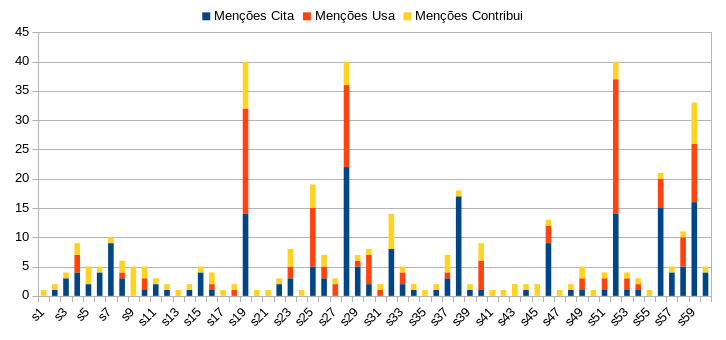
\includegraphics[scale=0.6]{imagens/mentions-by-type.png}
%  \caption{Menções por tipo de cada projeto.}
%  \label{mentions-by-type}
%\end{figure}
%
%\begin{figure}[h]
%  \center
  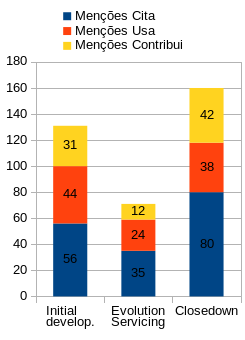
\includegraphics[scale=0.6]{imagens/mentions-stages-total.png}
  \caption{Total de menções por tipo em cada grupo de estágio distinto no ciclo de vida.}
  \label{mentions-stages-total}
\end{figure}

... a Figura \ref{closedown-mentions-vs-use} ... o projeto \texttt{s19}, \texttt{s38} e \texttt{s56} são
os com maior número de menções entre os projetos em estágio de {\it Closedown}, possuindo menções recentes
entre os anos de 2017, 2016 e 2014, respectivamente.

%\begin{figure}[h]
%  \center
%  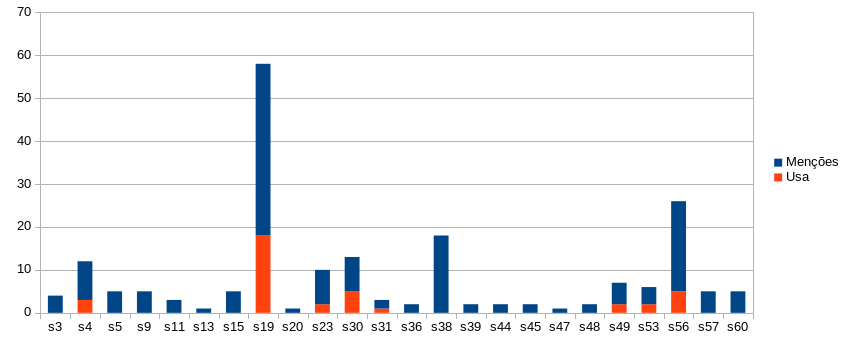
\includegraphics[scale=0.6]{imagens/closedown-mentions-vs-use.png}
%  \caption{Número total de menções em relaçao a menções do tipo {\it Usa} entre os projetos em estágio {\it Closedown}.}
%  \label{closedown-mentions-vs-use}
%\end{figure}

%Média de menções por grupo de estágio de evolução.
%
%\begin{figure}[ht]
%  \begin{minipage}{0.32\textwidth}
%    \centering
%    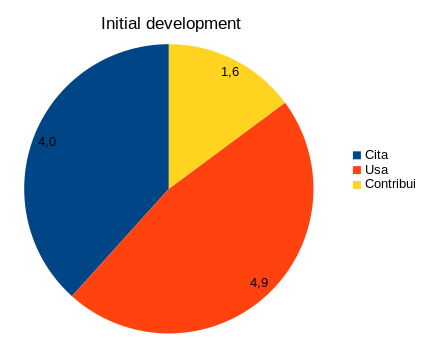
\includegraphics[scale=0.5]{imagens/mentions-initial-development.png}
%  \end{minipage}
%  \begin{minipage}{0.32\textwidth}
%    \centering
%    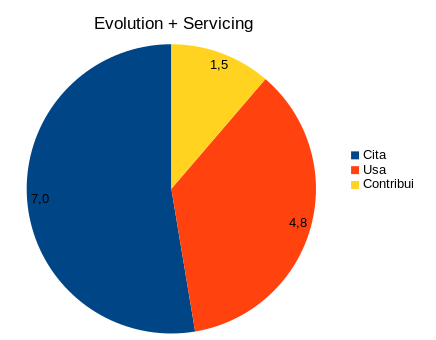
\includegraphics[scale=0.5]{imagens/mentions-evolution-servicing.png}
%  \end{minipage}
%  \begin{minipage}{0.32\textwidth}
%    \centering
%    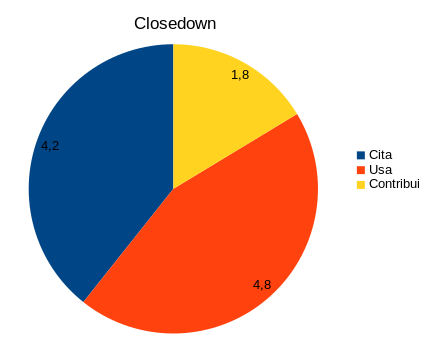
\includegraphics[scale=0.5]{imagens/mentions-closedown.png}
%  \end{minipage}
%  \caption{...}
%  \label{mentions-stages-blah}
%\end{figure}

  13 projetos foram encontrados num único e mesmo artigo já encontrado no estudo anterior
    (s1, s13, s17, s20, s21, s24, s35, s41, s42, s43, s47, s50, s55)
  47 foram encontrados em menções
    17 recebem contribuições
      (s4, s5, s8, s9, s10, s19, s23, s25, s26, s28, s32, s37, s40, s45, s49, s52, s59)

Entre os 24 projetos em estágio closedown encontramos 160 menções,
Entre os 8 em evolution+serving 71 menções,
Entre os 20 em initial encontramos 131 menções.

%      37 sem licença =       200 menções
%-38\% 23 com licença = +14\% 229 menções
%
%      24 sem download =       160 menções
%+50\% 36 com download = +68\% 269 menções
%
%19 projetos acima de 1 menção Contribui
%  260 menções ao total
%  184 lançamentos, 
%  7 closedown, 7 initial, 2 servicing
%
%39 projetos até 1 menção Contribui
%  169 menções
%  119 lançamentos
%  19 closedown, 2 evolution, 13 initial, 1 phaseout, 4 servicing

\subsection{Q5 - \QuestaoCinco} % evolução no tamanho

Initial apenas 55\% (11) são livres, evolution+servicing a maioria 87\% (7) são livres.

Entre os 60 projetos, 13 possuem baixo reconhecimento acadêmico (único artigo
mencionando é o artigo original publicando o software no ASE ou SCAM), entre
esses 10 tem download, 9 tem código, 5 initial, 2 evolução, 4 closedown, 1
phaseout, 1 unknown, 3 tem licença.

Entre os 60 projetos, 47 possuem maior reconhecimento acadêmico (foram
encontrados em mais artigos além da primeira publicação), entre estes 17 foram
mencionados em artigos fazendo contribuição, desses 17 10 tem download, 10 tem
código, 5 initial, 2 servicing, 7 closedown, 3 unknown, 8 tem licença.

Não há relação entre as características (número de lançamentos, tamanho em
módulos, licença, disponibilidade de download, etc) do projetos e o
reconhecimento acadêmico.



\begin{figure}[h]
  \center
  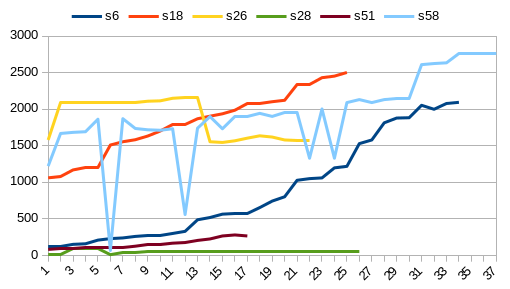
\includegraphics[scale=0.6]{imagens/modules-evolution-servicing.png}
  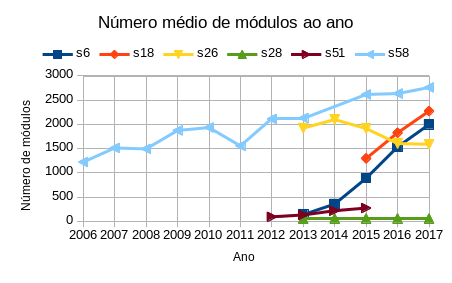
\includegraphics[scale=0.6]{imagens/modules-evolution-average.png}
  \caption{Evolução no número de módulos dos projetos em Servicing.}
  \label{modules-evolution-servicing}
\end{figure}

\subsection{Q6 - \QuestaoSeis}

...

\subsection{Q7 - \QuestaoSete}


\section{Trabalhos relacionados}

\citeonline{segal2008developing}
investigam como o desenvolvimento de software acadêmico pode ser melhorado e
enfatiza as diferenças do software acadêmico em relação aos demais tipos de
software, onde o conhecimento sobre o domínio pode muitas vezes incluir temas
avançados e pouco comuns fora do meio científico.

\citeonline{knutson2010report}
ao resumir as conclusões do evento RESER (Workshop on Replication in Empirical
Software Engineering Research) de 2011 cita que ferramentas de software
acadêmico estão indisponíveis ou não são usáveis em estágios não útil, tornando
replicação precisa impraticável.

\citeonline{robles2010replicating} num revisão de 171 artigos do MSR entre 2004 e 2009
em busca de conjunto de dados, artefatos e ferramentas utilizadas nos estudos
necessárias para replicação mostrou que a maioria dos artigos não conseguiram encontrar
as ferramentas mesmo quando o autor explicitamente afirma que fizeram uma.

%\citeonline{holcombe2011openaccess} no projeto {\it Open Access Pledge}
%\footnote{\url{http://www.openaccesspledge.com}} concentra-se em publicar
%softwares e papers em locais de {\it open access}.

\citeonline{portillo2012tools}
através de um mapeamento sistemático mostra que grande parte das ferramentas de
software criadas na academia estão em estado inicial de desenvolvimento que
apenas uma pequena porcentagem são testados fora do contexto onde foi
desenvolvido. 

\citeonline{chaturvedi2013tools}
faz uma revisão de literatura entre artigos submetidos ao MSR de 2007 até 2013,
identifica conjunto de dados, ferramentas e técnicas utilizadas pelos autores,
mais da metade dos artigos usam ou criam ferramentas, categoriza as ferramentas
em ferramentas novas, ferramentas tradicionais, protótipos e scripts para
mineração de dados.

\citeonline{barnes2013science}
cria o manifesto {\it Science Code Manifesto} e enfatiza que todo código fonte
escrito especificamente para processar dados de publicações devem estar
disponíveis aos revisores e leitores do paper.

\citeonline{marshall2013tools} num mapeamento sistemático sobre artigos criando
ferramentas de apoio a revisão sistemática no domínio de SE conclui que as
ferramentas encontradas estão em estado inicial de desenvolvimento.

\citeonline{hettrick2014uk} mostra que no reino unido entre todas as áreas da
ciência 56\% dos cientistas estão envolvidos no desenvolvimento de software
acadêmico.

\citeonline{wilson2014best} resume as melhores práticas para melhoria da
manutenibilidade e disponibilidade do software acadêmico desenvolvido por
cientistas.

\citeonline{wilson2014software} num resumo sobre as lições aprendidas em 20
anos da iniciativa {\it Software Carpentry} sobre atividades de melhoria das
habilidades dos pesquisadores com computacao.

\citeonline{amann2015software}
investigam através de uma revisão sistemática de literatura uma década de
publicações e encontram que muito poucos estudos são replicáveis visto que
faltam informações incluindo dados e ferramentas, apenas 20\% dos estudos
possuem ferramentas disponíveis.

\citeonline{momcheva2015software}
num survey com 1142 participantes sobre o uso de software em pesquisas da
astronomia mostrou que 90\% dos cientistas escrevem software e 100\% usam
software em suas pesquisas.

\citeonline{beller2016analyzing} avalia e sugere caminhos para melhorar o
desenvolvimento de ferramentas de análise estática com o objetivo de aumentar a
adoção.

\citeonline{smith2016software} resume recomendações sobre como citar software
na literatura acadêmica com objetivo de encorajar uma ampla adoção e uma
política consistente para citação de software entre as múltiplas disciplinas.

\citeonline{smith2016software} afirma que ``citações aos softwares devem
permitir e facilitar acesso ao software, metadados, documentação, dados e
outros materiais necessários tanto para humanos quanto para máquinas''.

%\citeonline{wilkinson2016fair} através do {\it FAIR
%principles}\footnote{\url{https://www.nature.com/articles/sdata201618}} com
%foco em dados de pesquisa, o objetivo é fazer eles serem encontráveis,
%acessíveis, interoperável e reusável. Estes princípios podem ser generalizados
%para aplicar aos softwares.

\citeonline{howison2016software}
numa revisão de literatura mostrou que publicações usando softwares como
método, mostrou que apenas 59 mencionavam o uso de softwares de alguma forma,
os demais 31 artigos, apesar de usar software acadêmico, não mencionavam nada a
respeito.

\citeonline{wilson2017good} apresenta um conjunto de boas práticas que todo
pesquisador pode adotar, independentemente do seu nível de habilidade em
computação. Essas práticas passam por gerenciamento de dados, programação,
colaboração com colegas, organização de projetos, tracking work, e escrita da
manuscritos.
%, sao desenhados para uma grande variadade de fontes publicadas do
%noso dia a dia e do nosso trabalho como voluntário organizando workshopts desde
%2010.

%Open Science Peer Review Oath\footnote{\url{https://f1000research.com/articles/3-271/v2}}
%Concentra-se em potencializar os revisores para exigir acesso aberto aos
%softwares, práticas reprodutíveis e revisões transparentes.

%Muitos pesquisadores não
%disponibilizam os seus softwares 
 %ou quanto o fazem enfrentam problemas com disponibilidade e
%manutenibilidade \cite{prlic2012ten}
